%================================================================================================================================================
\subsection{Verwendung von Bildern}
Die verbale Darstellung von Informationen ist zwar exakt aber nicht sehr anschaulich.
Nach dem Prinzip "`ein Bild sagt mehr als tausend Worte"' können viele Sachverhalte einfacher und klarer in Form von Bildern dargestellt werden als es durch verbale Beschreibung möglich ist.
Die Inhalte sollten grafisch dargeboten werden, weil sie so leichter aufgenommen und verarbeitet werden können \cite[S.~67]{Hering2009}.
Es ist wichtig eine geeignete Darstellungsform für die Veranschaulichung der theoretischen Inhalte zu finden.
Dies müssen nicht unbedingt Abbildungen, sondern können auch Tabellen, Diagramme oder andere Darstellungsformen sein.

"`Grafiken, Tabellen und Fotos, die aus einer fremden Quelle übernommen wurden, müssen mit einem entsprechenden Verweis auf den Ursprung versehen werden.
Eigenerstellte Inhalte werden nicht explizit gekennzeichnet"' \cite[S.~111]{Balz2008}.
Wie in Abbildung \ref{fig:KompassSensor} zu sehen ist, setzt sich die Abbildungsunterschrift aus Nummerierung, gefolgt von der Benennung und der Quellenangabe zusammen. 
Bei der Abbildungsunterschrift sowie Tabellenüberschriften wird auf das Satzzeichen am Ende des Satzes verzichtet.
In der Regel gilt bei Abbildungen und Tabellen eine horizontal zentrierte Anordnung, da das optische Erscheinungsbild dadurch ausgewogen erscheint \cite[S.~183]{Balz2008}.
Für die Abbildungsunterschrift sowie Tabellenüberschrift gilt ebenfalls eine zentrierte Anordnung.

\begin{figure}[h]
	\centering
		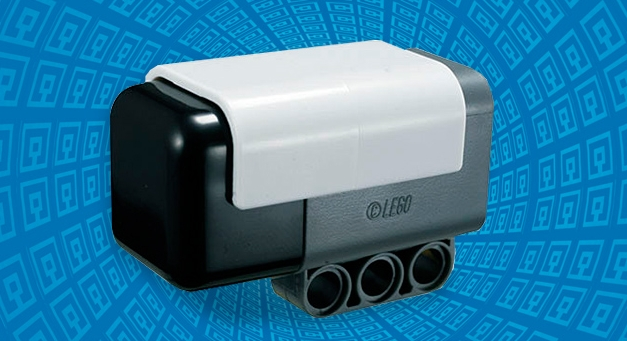
\includegraphics[width=0.5\textwidth]{KompassSensor.jpg}\\
			\caption{Kompasssensor für Lego Mindstorms NXT und EV3 \cite{Lego12}}
		\label{fig:KompassSensor}
\end{figure}

\noindent
Bilder und Tabellen werden entweder durch die ganze wissenschaftliche Ausarbeitung chronologisch durchnummeriert wie es in dieser wissenschaftlichen Arbeit gehandhabt wird.
Oder die Nummern werden aus der Kapitelnummer und einer laufenden Nummer innerhalb des Kapitels kombiniert \cite[S.~15]{Hering2009}.

Jede Abbildung muss als Querverweis im Text referenziert werden \textbf{bevor} diese im Dokument erscheint.
Auf jedes Bild muss im Text mindestens einmal hingewiesen werden.
Dabei soll eine Verbindung zwischen Bild und Text geschaffen werden und das Bild möglichst in der Nähe des Hinweises im Text erscheinen.
Falls von mehreren Stellen auf ein Bild hingewiesen wird, dann sollte das Bild in der Nähe des wichtigsten Hinweises angeordnet werden \cite[S.~76]{Hering2009}.

Bei der Auswahl der Abbildung muss darauf geachtet werden, dass diese in angemessener Druckqualität vorliegt.
Die Qualität kann durch ein Bildbearbeitungsprogramm optimiert werden, indem der Kontrast oder die Schärfe angepasst wird.
Grundsätzlich sollte eine Abbildung nur Informationen beinhalten, die im Text beschrieben werden.
Damit das Bild übersichtlich bleibt, sollte in Abbildungen nur das Wesentliche dargestellt werden.
Durch das Weglassen und Vereinfachen von Elementen in der Abbildung wird beim Leser die Konzentration auf das Wesentliche gelenkt \cite[S.~70~f.]{Hering2009}.

Der Übersichtlichkeit halber sollten auf einer Textseite nicht mehr als zwei Abbildungen, Tabellen oder andere Visualisierungsformen abgebildet werden.
Generell sollten Abbildungen nur dann eingesetzt werden, wenn es notwendig ist, komplexe Inhalte darzustellen, nicht als bloße Dekoration.
Wenn innerhalb der Abbildung schriftliche Anteile enthalten sind, sollte die Schriftgröße leserlich oder optimalerweise so groß wie die verwendete Schriftgröße im Text sein.
Es sollte vermieden werden, dass ein Bild unbekannte Fachbegriffe enthält oder dass in Text und Bild unterschiedliche Bezeichnungen für gleiche Gegenstände oder Sachverhalte auftreten \cite[S. 80]{Hering2009}.
